\documentclass{exam}

\usepackage{units} 
\usepackage{graphicx}
\usepackage[fleqn]{amsmath}
\usepackage{cancel}
\usepackage{float}
\usepackage{mdwlist}
\usepackage{booktabs}
\usepackage{cancel}
\usepackage{polynom}
\usepackage{caption}
\usepackage{fullpage}
\usepackage{xfrac}
\usepackage{enumerate}

\newcommand{\degree}{\ensuremath{^\circ}} 
\everymath{\displaystyle}

\printanswers

% \begin{figure}[H]
%   \centering
%   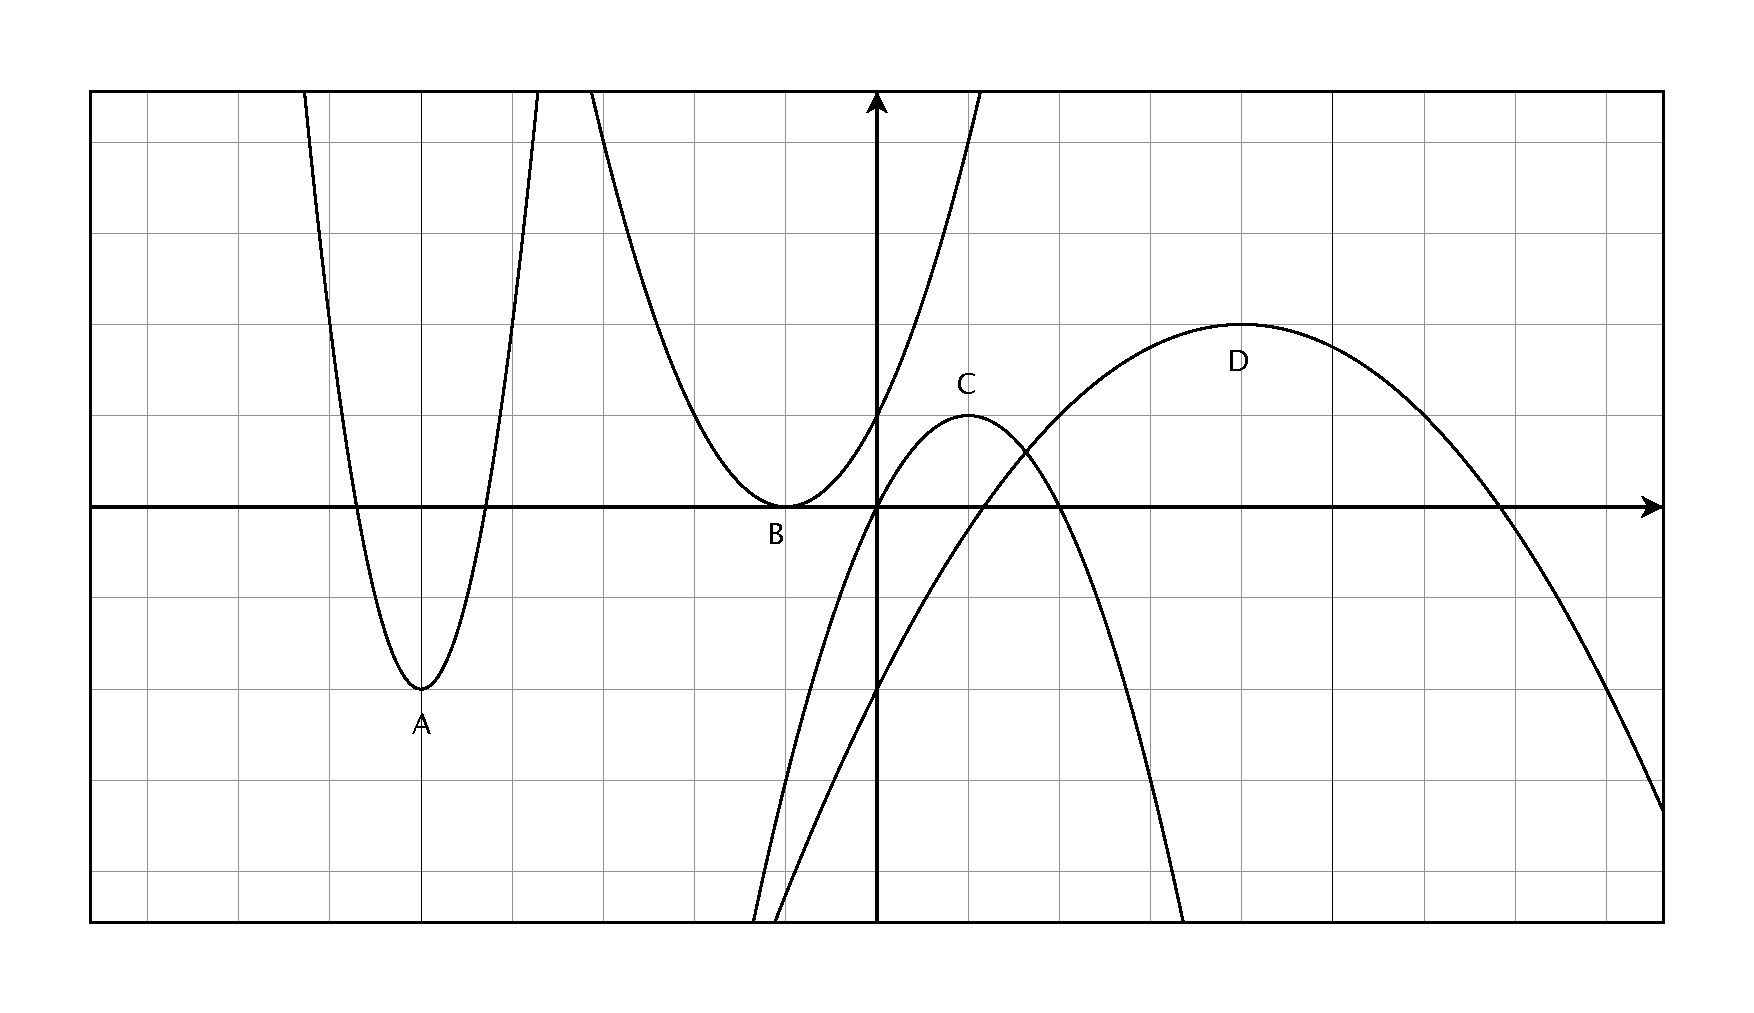
\includegraphics[scale=.3]{problem_7.eps}
%   \caption*{Problem 7}
% \end{figure}

% \begin{tabular}{cc}
% \toprule
% period & amplitude \\
% \midrule
%   $\pi$ & $2$ \\
% \bottomrule
% \end{tabular}

\title{Math 141 Notes \\ Chapter Two Review}
\date{February 27, 2013}

\begin{document}

\maketitle
\tableofcontents

\section{Homework 5 Notes}
\begin{itemize}
  \item For composition of functions, the final domain must take into consideration the original domains.  This is true
    even if things cancel so values which weren't valid in the original domain are valid in the final domain.  For
    example:
    \begin{align*}
      f(x) &= \sqrt{x + 1} \\
      g(x) &= x^2 \\
      (g \circ f)(x) &= x + 1 \\
    \end{align*}

    The domain of $g \circ f$ is $(-1, \infty)$

  \item When trying to think of how to make a function by composing two other functions, it isn't fair to use $f(x) = x$
    for one of the functions and the original function as the other function.

  \item Show your work and keep your homework in case EdCC wants to see it later.

  \item Do extra credit problems in class.

\end{itemize}

\section{Proof of the Day}
\[
  \sum_{i = 1}^n = \frac{n(n + 1)}{2}
\]

\section{Function Composition Applications}
\begin{enumerate}
  \item Sand is pored into a conical pile whose radius and height are always equal, although both increase with time.
    The height of the pile $\unit[t]{seconds}$ after pouring begins is given by $h(t) = \unit[10 + 0.25t]{ft}$.  Express the
    volume of the pile as a function of $t$.

    The volume of a cone is $v = \frac{1}{3} \pi r^2 h$.

    \begin{solution}
      \begin{align*}
         v &= \frac{1}{3} \pi h^3 \\
       &= \frac{1}{3} (10 + 0.25t)^3 \\
      \end{align*}
    \end{solution}

  \item Tax Rates
    Alice has a mortgage and 401(k) plan.  She is in the 30\% tax bracket and pays 6\% Social Security tax on the first
    \$100,000 of her income, which is more than \$100,000.  She also spends 20\% of her income on taxable items which
    are taxed by the WA state sales tax of 10\%.

    Bob rents, is in the 25\% tax bracket and doesn't have a 401(k) plan.  He makes less than \$100,000 and spends 50\%
    of his income on taxable items.

    Find functions for each person's tax rate.  If Alice makes \$150,000 and Bob makes \$50,000, find their tax rates.

    \begin{solution}
      \begin{itemize}
        \item Alice's taxable income is: $A(x) = x - 15000 - 15000$
        \item Alice's tax, as a function of income is: $T(i) = 0.3i + 0.02i + 6000 = 0.32i + 6000$
        \item Alice's tax rate is $R \circ T \circ A$.
        \item Bob's taxable income is: $B(x) = x$
        \item Bob's tax rate is: $T(i) = 0.25i + 0.05i + 0.06i = 0.36i$
      \end{itemize}

      \begin{itemize*}
        \item Alice's effective tax rate is 30\%.
        \item Bob's effective tax rate is 36\%.
      \end{itemize*}
    \end{solution}
    
  \item A spherical balloon is inflated so that its radius at the end of $\unit[t]{seconds}$ is 
    \[
      r(t) = \unit[3 \sqrt{t} + 5]{cm}
    \]

    Express the volume and the surface area as functions of time.

    \begin{solution}
      \begin{align*}
        V(t) &= \frac{4}{3} \pi r^3 \\
        A(t) &= 4 \pi r^2 \\
      \end{align*}
    \end{solution}

\end{enumerate}


\section{Miscellaneous}

Talk to Jeff Grote about 
\begin{itemize*}
  \item piecewise defined functions
  \item sign charts
\end{itemize*}

\end{document}
